\section{Theoretical Framework}
\label{Theoretical Framework}

\subsection{Topic Modeling - Overview}
\label{Topic Modeling - Overview}

Topic models seek to discover latent thematic clusters, called topics, within a collection of discrete data, usually text; therefore, topic modeling can be regarded as dimensionality reduction technique. Furthermore, since both the number and content of topics is unknown beforehand (and can never be truly verified), topic modeling is an instance of unsupervised learning. Information retrieval (IR) research generally proposes the reduction of text documents to vectors of real numbers, each number representing (modified) counts of or terms. An instance of this proposed methodology is the \textit{tf-idf} scheme by \cite{salton1983information}, which for a collection of documents returns a term-by-document matrix where each row corresponds to a document in the corpus and the columns contain the respective \textit{tf-idf} term count. Since only words in a vocabulary of fixed length $V$ are considered, documents of unrestricted length are being reduced to vectors of a fixed length $V$. To further reduce dimensionality, the \textit{latent semantic indexing} (LSI) by \cite{deerwester1990indexing} applied singular value decomposition (SVD) to the \textit{tf-idf} document-term matrix. However, as \cite{blei2003latent} argue, the idea should be to develop a generative probabilistic model of text, in order to estimate to which extent the LSI methodology can align data with the generative text model; yet, given such a model, Bayesian methods or maximum likelihood estimation (MLE) would be much more direct, which is why the benefits of applying the LSI are not obvious. Picking up this shortcoming of LSI, \cite{hofmann1999probabilistic} introduced the \textit{probabilistic LSI} (pLSI) model. This generative data model allows for individual words to be sampled from a mixture model: they are drawn from a multinomial distribution, with latent random variables determining the mixture proportions, which in turn can be viewed as topics. However, the pLSI can only be regarded as partly probabilistic text model, since the mixing components themselves are fixed on a document level, thus lacking a probabilistic generating process.

In their \textit{Latent Dirichlet Allocation} (LDA) model, \cite{blei2003latent} included the generation of topic proportions into the generative probabilistic model, the resulting three-level hierarchical Bayesian mixture model marking the starting point of modern topic modeling. In order to present the main idea of LDA, we first introduce some notation and terminology that we will use throughout the remainder of this paper.

\begin{itemize}
\vspace{-0.25cm}
\item[•] A \textit{word} is the smallest unit of discrete text data. Words are instances of a vocabulary of $V$ unique \textit{terms} and can thus be indexed by $v \in \{1,\dots,V\}$. Mathematically, the $v$-th term in the vocabulary can be represented as a vector of length $V$, whose $v$-th component equals one, with all other components equalling zero. We will sometimes refer to the $v$-th term of the vocabulary simply as $v$. Words, along with document-level metadata, represent the actually observable data.
\vspace{-0.25cm}
\item[•] A \textit{document} $d \in \{1,\dots,D\}$ is a sequence of words of length $N_{d}$. For a given document $d$, we denote its words by $(w_{d,1},\dots,w_{d,N_{d}})$. Consequently, the $n$-th word of document $d$ is denoted by $w_{d,n}$.
\vspace{-0.25cm}
\item[•] A \textit{corpus} is a collection (or set) of $D$ documents. Therefore, $d \in \{1,\dots,D\}$ means that our corpus contains $D$ documents.
\vspace{-0.25cm}
\item[•] A \textit{topic} is a latent thematic cluster within a text corpus. The idea is that any collection of documents is made up of $K$ such topics, where the number of topics $K$ is an (unknown) hyperparameter which needs to be determined ex ante (see section \ref{Hyperparameter Search and Model Fitting} for hyperparameter determination in our specific use case). We will refer to topics simply by the actual \textit{topic index} (or \textit{topic number}) $k \in \{1,\dots,K\}$.
\vspace{-0.25cm}
\item[•] A \textit{topic-word distribution} $\boldsymbol{\beta}$ is a probability distribution over words, i.e., over the vocabulary. For a model containing $K$ topics (and no topical content variable, see section \ref{The Structural Topic Model} below), topic-word distributions do not vary across documents and uniquely characterize a topic: we denote the word distribution corresponding to the $k$-th topic by $\boldsymbol{\beta}_k$ and the matrix whose $k$-th column is topic $\boldsymbol{\beta}_k$ by $\boldsymbol{B}:=\boldsymbol{\beta}_{1:K}=[\boldsymbol{\beta}_1|\dots|\boldsymbol{\beta}_K]$. Each vector $\boldsymbol{\beta}_k$ thus has length $V$, while $B$ is a $V \times K$-matrix. Therefore, $k$ refers to the latent thematic cluster with topic index $k$ in general, and $\boldsymbol{\beta}_k$ refers to the underlying word distribution in particular.
\vspace{-0.25cm}
\item[•] A \textit{topic assignment} $\boldsymbol{z}_{d,n}$ is the assignment of the $n$-th word of document $d$ to a specific topic $k \in \{1,\dots,K\}$ (i.e., to the corresponding word distribution $\boldsymbol{\beta}_k$). Therefore, $\boldsymbol{z}_{d,n}$ is simply a vector of length $K$ whose $k$-th entry equals one and all other entries equal zero. This allows us to represent the word distribution corresponding to the $n$-th word in document $d$ as $\boldsymbol{\beta}_{d,n}:=B\boldsymbol{z}_{d,n}$ (again, for a model without topical content variable).
\vspace{-0.25cm}
\item[•] For a given document $d$, the corresponding \textit{topic proportions}, denoted by $\boldsymbol{\theta}_d$, are the proportions of the document's terms assigned to each of the topics $k \in \{1,\dots,K\}$. Topic proportions vary across documents. Since for each document $d$ the proportions of all $K$ topics must add up to one ($\sum_{k=1}^{K}\theta_{d,k}=1$, for all $d \in \{1,\dots,D\}$), topic proportions represent probabilities.
\vspace{-0.25cm}
\item[•] The \textit{bag-of-word} assumption is an assumption used in all (probabilistic) text models referenced in this paper, including LSI and pLSI, and states that only words themselves (and their counts) carry meaning, while word order or grammar do not. Statistically, this is equivalent to assuming that words within a document are \textit{exchangeable} (\citealp{aldous1985exchangeability}).

\end{itemize}

As mentioned above, LDA is the first generative probabilistic model of an entire text corpus. (Recall that pLSI is only probabilisitic for a fixed document.) 
Now, the generative process underlying LDA can be described as a two-step procedure, where for each document $d \in \{1,\dots,D\}$:

\begin{enumerate}[{1)}]
\vspace{-0.25cm}
\item Draw topic proportions $\boldsymbol{\theta}_d \sim \text{Dir}_K(\boldsymbol{\alpha})$.
\vspace{-0.25cm}
\item For each word $n \in \{1,\dots,N_d\}$:
	\begin{enumerate}[{a)}]
	\vspace{-0.25cm}    
    \item Draw a topic assignment $\boldsymbol{z_{d,n}} \sim \text{Multinomial}_K(\boldsymbol{\theta}_d)$.
	\vspace{-0.25cm}    
    \item Draw a word $w_{d,n} \sim \text{Multinomial}_V(\boldsymbol{\beta}_{d,n})$.
	\end{enumerate}
\end{enumerate}

\noindent
Thus, topic proportions are drawn from a Dirichlet distribution with $K$-dimensional $\boldsymbol{\alpha}$, with all components $\alpha_k > 0$, where the number of topics $K$ is a hyperparameter to be set by the user; the $\boldsymbol{\alpha}$-vector is estimated from the data. This means that for each document $d \in \{1,\dots,D\}$, the corresponding topic proportions $\boldsymbol{\theta}_d$ represent a $K$-dimensional vector which can take on values on the ($K-1$)-simplex, i.e., $\theta_{d,k} \geq 0, \sum_{k=1}^{K}\theta_{d,k}=1$. Also note that the Dirichlet distribution is the conjugate prior of the multinomial distribution, which greatly facilitates estimation (see section \ref{Inference and Parameter Estimation} on variational inference below). Put simply, for each document LDA first generates topic proportions, which are then used as weights for topic assignment. A word is then drawn from a topic-specific word distribution, which is determined by the topic assignment. These topic-specific word distributions $\boldsymbol{\beta}_k$ need to be estimated from data.
Note that LDA is a very simple, restrictive model in (at least) three ways:

\begin{enumerate}[label=(\roman*)]
\vspace{-0.25cm}
\item By using the Dirichlet distribution to generate topic proportions, potential correlations between topics cannot be captured due to the neutrality of the Dirichlet distribution.\footnote{Due to the constraint $\sum_{k=1}^{K}\theta_{k}=1$, there is clearly some degree of dependence between topic proportions. However, the dependence is minimal, as the Dirichlet distribution is characterized by complete neutrality: the components $\theta_1/(1-S_0), \theta_2/(1-S_1),\dots, \theta_K(1-S_{K-1})$ are mutually independent, where $S_0:=0$ and $S_k = \sum_{i=1}^{k}\theta_k, k \in \{1,\dots,K\}$. Stated differently, for each component $\theta_k, k \in \{1,\dots,K\}$, it holds that $\theta_k/(1-S_{k-1})$ is independent of the vector constructed by weighting all \textit{remaining} components by their total proportion (\citealp{james1980new})}. As a consequence, the occurrence of one topic within a document is not correlated with the occurrence of another topic (\citealp{blei2007correlated}). This is a restrictive simplification, as topics such as "sports" and "health" are much more likely to co-occur within a document than, say, "sports" and "war".
\vspace{-0.25cm}
\item Second, while topic proportions vary stochastically across documents, they do so given a single, global hyperparameter vector $\boldsymbol{\alpha}$; recalling the bag-of-words assumption, this implies that topic proportions are generated based merely on word counts (occurrences and co-occurrences), while additional document-level information is not taken into account. This is another unrealistic and limiting simplification, since researchers usually possess further document-specific information indicative of the topics addressed within the individual documents.
\vspace{-0.25cm}
\item Third, by construction, the topic-specific word distributions $\boldsymbol{\beta}_k$ are assumed to be identical for all documents. Similarly to the second restriction, this prevents researchers from using (document-level) information which might potentially influence the weighting of specific words within a topic.

\end{enumerate}

\noindent
Due to its simplicity and the resulting restrictions, the LDA has been used used as a building block for more advanced (and usually more specified) generative topic models. One model that builds on LDA, addressing some of its shortcomings, is the \textit{Correlated Topic Model} (CTM) by \cite{blei2007correlated}. Specifically, the CTM addresses the first one of the abovementioned restrictions: the inability to cope with inter-topic correlations. The model no longer uses a Dirichlet distribution to sample topic proportions; instead, a logistic normal distribution is employed, which can capture correlations between topics due to the incorporated covariance structure between its components (\citealp{atchison1980logistic}). The resulting generative process for the CTM can be stated as follows:

\vspace{0.25cm}
\noindent
For each document $d \in \{1,\dots,D\}$:

\begin{enumerate}[{1)}]
\vspace{-0.25cm}
\item Draw unnormalized topic proportions $\boldsymbol{\eta}_d \sim \mathcal{N}_{K-1}(\boldsymbol{\mu}, \boldsymbol{\Sigma})$, with $\eta_{d,K} := 0$ for model identifiability.
\vspace{-0.25cm}
\item Normalize $\boldsymbol{\eta}_d$ by mapping it to the simplex: $\theta_{d,k} = \frac{exp(\eta_{d,k})}{\sum_{j=1}^{K}exp(\eta_{d,j})}$, for all $k \in \{1,\dots,K\}$.
\vspace{-0.25cm}
\item For each word $n \in \{1,\dots,N_d\}$:
	\begin{enumerate}[{a)}]
	\vspace{-0.25cm}    
    \item Draw a topic assignment $\boldsymbol{z_{d,n}} \sim \text{Multinomial}_K(\boldsymbol{\theta}_d)$.
	\vspace{-0.25cm}    
    \item Draw a word $w_{d,n} \sim \text{Multinomial}_V(\boldsymbol{\beta}_{d,n})$.
	\end{enumerate}
\end{enumerate}

\noindent
The first two steps constitute the sampling from a logistic normal distribution: a $K$-dimensional vector $\boldsymbol{\eta}_d$ is drawn from a multivariate normal distribution and subsequently transformed to a vector of proportions (or probabilities) by applying the \textit{softmax} function to each of its elements. The number of topics $K$ is again a hyperparameters which must be determined ex ante. As in LDA, the parameters of the normal distribution in step 1, $\boldsymbol{\mu} \in \mathbb{R}^{K-1}$ and $\boldsymbol{\Sigma} \in \mathbb{R}^{(K-1) \times (K-1)}$, as well as the topic-specific word distributions $\boldsymbol{\beta}_k$ need to be estimated from the data. As mentioned above, this process now allows for inter-topic correlation. Yet this comes at a cost: unlike the Dirichlet distribution, the logistic normal distribution is no longer conjugate to the multinomial distribution. As explained in more detail in section \ref{Inference and Parameter Estimation} below, this renders standard variational inference algorithms inapplicable, since these rely on conjugacy and the implied closed-form solutions. However, using the Laplace variational inference developed by \cite{wang2013variational}, which is a generic method for variational inference when dealing with nonconjugate models, solves the inference problem for the CTM.

As for the inability to integrate covariate information into the determination of topic proportions, \cite{mimno2011optimizing} were the first to model topic proportions as a function of \textit{observable} document-level metadata. Specifically, their \textit{Dirichlet-Multinomial Regression} (DMR) model still samples topic proportions $\boldsymbol{\theta}_d$ from a Dirichlet distribution (thus, not allowing for inter-topic correlations), yet unlike in LDA, the Dirichlet prior $\boldsymbol{\alpha}_d$ is no longer global but topic-specific. This topic prior $\boldsymbol{\alpha}_d$, in turn, is log-linear in the document-level features $\boldsymbol{x}_d$ and the (topic-specific) priors for the coefficients of these features, $\boldsymbol{\lambda}_t$, have a normal prior. With coefficients being updated through numerical optimization as part of the EM algorithm used for training, the DMR model thus actively uses document features to model topic proportions. 

Finally, the third restictiveness of LDA, the inflexibility of the topic-word distributions $\boldsymbol{\beta}_k$ when document-level metadata is available, is addressed by \cite{eisenstein2011sparse} in their \textit{Sparse Additive General} model (SAGE). The authors propose to start off with a background word distribution $m$ containing log frequencies and to model additive deviations from this baseline for each class. The idea behind SAGE can be used to model differences in topic-word distributions according to the category of some document-level covariate.

Based on the foundational LDA as well as its extensions, \cite{roberts2013structural} developed the \textit{Structural Topic Model} (STM), which combines the improvements over the original LDA discussed in this section. Due to its flexibility regarding the incorporation of document-level information, we choose the STM for our specific use case, a text-based analysis of German political entities (TBD, depends on final title of paper). Therefore, we discuss the model in greater detail in section \ref{The Structural Topic Model} below.

\subsection{The Structural Topic Model}
\label{The Structural Topic Model}

\subsubsection*{Overview}

The STM addresses the three main shortcomings of the LDA, as discussed in the previous section. In this subsection, we explain the corresponding modifications with respect to LDA and present the generative process of the STM.

\begin{enumerate}[label=(\roman*)]
\vspace{-0.25cm}
\item To allow for correlation among topics, the STM uses a logistic normal distribution to sample topic proportions. In fact, if no document-level metadata is fed into the STM, it simply reduces to the CTM.
\vspace{-0.25cm}
\item The STM allows for the incorporation and use of document-level metadata when determining topic proportions. Similar to the DMR, topic proportions $(\boldsymbol{\theta}_1,\dots,\boldsymbol{\theta}_D)^T$ are assumed to depend on $P$ document-level \textit{topical prevalence variables} (such as the author's name, her political party or her popularity on Twitter), yet now with each $\boldsymbol{\theta}_d$ following a multivariate logistic normal distribution. The distribution now has median vector\footnote{There is no analytical closed form for the mean in the logistic normal distribution.} $\boldsymbol{\Gamma}^T\boldsymbol{x_d}^T$; $\boldsymbol{X}=[\boldsymbol{x_1}|\dots|\boldsymbol{x_D}]^T \in \mathbb{R}^{D \times P}$ is a matrix containing $D$ document-level prevalence covariate vectors $\boldsymbol{x}_d$, each one containing $P$ document-level covariate values; $\boldsymbol{\Gamma} = [\boldsymbol{\gamma}_1|\dots|\boldsymbol{\gamma}_K]$ is a matrix with each of its $K$ columns $\boldsymbol{\gamma}_k$ being a $P$-dimensional vector of topic proportion coefficients for the respective topic $k$. Furthermore, $\boldsymbol{\Sigma}$ is a matrix of parameters determining the covariance structure of the distribution (for details see further below). This way, the model accounts for the fact that document-level covariates might influence how much (that is, which percentage of the total number of words) the corresponding documents attribute to the different topics.
\vspace{-0.25cm}
\item Within the STM, document-level covariate information can also be used to fine-tune the topic-word distributions $\boldsymbol{\beta}_k$, the methodology being similar to the one in the SAGE model. In particular, the STM allows for specifying a single categorical document-level \textit{topical content variable} $\boldsymbol{Y}\in \mathbb{R}^D$ with $A$ levels, i.e., $Y_d \in \{1,\dots,A\}$, for all $d \in \{1,\dots,D\}$ (\citealp{stm}).\footnote{In theory, multiple topical content variables could be included, yet the R package \textbf{stm} (\citealp{stm}) only allows for specifying a single content variable due to computational complexity. Furthermore, $Y_d$ is dummy encoded in the model implementation, making $Y_d$ a vector of length $A$ and $\boldsymbol{Y}$ a matrix of dimension $D \times A$. However, for notational convenience we simply refer to $Y_d$ as a scalar and to $\boldsymbol{Y}$ as a $D$-dimensional vector here.} Consequently, each topic $k \in \{1,\dots,K\}$ is now associated with a total of $A$ topic-word distributions $\boldsymbol{\beta}_{k,a}, a \in \{1,\dots,A\}$ instead of a single one, $\boldsymbol{\beta}_k$. For a given document $d$, this means the $K$ topic-word distributions are now additionally determined by the level $a$ assumed by $Y_d$ and are identical across all documents with $Y_d = a$, given a topic $k \in \{1,\dots,K\}$ (\citealp{roberts2016model}). This way, for a given document $d$, document-level metadata can not only impact the weighting of topics $\boldsymbol{\theta}_d$, but also the weighting over words for each topic. Note that for a given topic $k$, the word distributions $\boldsymbol{\beta}_{k,a}$ do not vary substantially across different values of $a$; that is, the content variable $\boldsymbol{Y}$ is really an $A$-level refinement of $\boldsymbol{\beta}_k$ and does \textit{not} affect the number of topics $K$.

\end{enumerate}

\noindent
The generative process of the STM can be stated as follows (\citealp{roberts2016model}):

\vspace{0.25cm}
\noindent
For each document $d \in \{1,\dots,D\}$:

\begin{enumerate}[{1)}]
\vspace{-0.25cm}
\item Draw unnormalized topic proportions $\boldsymbol{\eta}_d \sim \mathcal{N}_{K-1}(\boldsymbol{\Gamma}^T\boldsymbol{x_d}^T, \boldsymbol{\Sigma})$, with $\eta_{d,K}$ set to zero for model identifiability.
\vspace{-0.25cm}
\item Normalize $\boldsymbol{\eta}_d$ by mapping it to the simplex: $\theta_{d,k} = \frac{exp(\eta_{d,k})}{\sum_{j=1}^{K}exp(\eta_{d,j})}$, for all $k \in \{1,\dots,K\}$.
\vspace{-0.25cm}
\item For each word $n \in \{1,\dots,N_d\}$:
	\begin{enumerate}[{a)}]
	\vspace{-0.25cm}    
    \item Draw a topic assignment $\boldsymbol{z_{d,n}} \sim \text{Multinomial}_K(\boldsymbol{\theta}_d)$.
	\vspace{-0.25cm}    
    \item If no topical content variable has been specified, simply draw a word $w_{d,n} \sim \text{Multinomial}_V(\boldsymbol{\beta}_{d,n})$. Otherwise, first determine the document-specific word distributions $B_a := [\boldsymbol{\beta}_{1,a}|\dots|\boldsymbol{\beta}_{K,a}]$ based on the level $a$ taken on by $Y_d$, for all topics $k \in \{1,\dots,K\}$; next, analogously define $\boldsymbol{\beta}_{d,n}:=B_a\boldsymbol{z_{d,n}}$; finally, draw a word $w_{d,n} \sim \text{Multinomial}_V(\boldsymbol{\beta}_{d,n})$.
	\end{enumerate}
\end{enumerate}

\noindent
This means that unnormalized topic proportions are sampled from a normal distribution with mean $\boldsymbol{\Gamma} = [\boldsymbol{\gamma}_1|\dots|\boldsymbol{\gamma}_K]$ and covariance $\boldsymbol{\Sigma}$. The coefficients contained in the matrix $\boldsymbol{\Gamma}$, which correspond to the prevalence covariates $\boldsymbol{X}$, are obtained through a Bayesian linear regression with prior distributions $\boldsymbol{\gamma}_k \sim \mathcal{N}_p(0, \sigma_k^2\boldsymbol{I}_p)$ (see \citealp{roberts2016model} for further details). However, we actually specify an L1 penalty instead of this prior to ensure model convergence. The softmax function is then applied to unnormalized topic proportions $\boldsymbol{\eta}_d$, yielding normalized topic proportions $\boldsymbol{\theta}_d$, which in turn are used as weights for the subsequent topic assignment $\boldsymbol{z_{d,n}}$. Finally, each word is sampled from the corresponding multinomial word probability distribution (over the vocabulary of length $V$), which depends on topic assignment $\boldsymbol{z_{d,n}}$ and, for models containing a topical content variable, on its level $a$. In line with SAGE methodology, the topic-word distributions are modelled as deviations in log-frequency from a baseline vocabulary. (See \citealp{roberts2016model}, p.\ 991 for more details.) As in the CTM, $K$ (and $\sigma_k^2$ if no L1 penalty is specified) is a hyperparameter to be chosen by the user. The graphical model representation in Figure 1 below visualizes the generative process described.


\begin{figure}[h!]
  \centering
  \captionsetup{justification=centering,margin=2cm}
  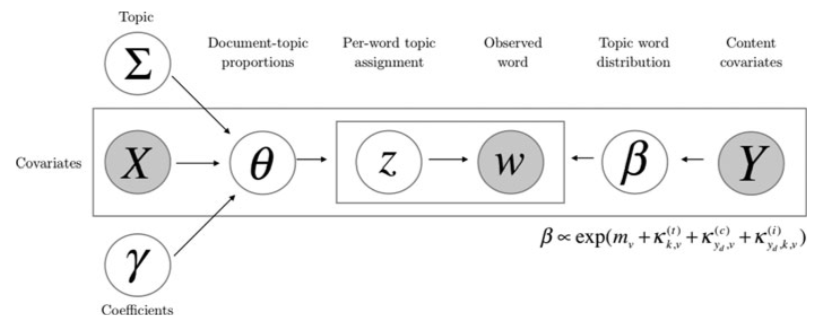
\includegraphics[scale = 0.5]{../plots/2/stm_graphical.png}
  \caption{Graphical model representation of the STM (from \cite{roberts2016model}, p.\ 990).}
  \label{fig:graphical_model}
\end{figure}

\subsubsection*{Scope}

Topic models are unsupervised learning methods, since the true topics from which the text was generated are not known. They have been traditionally used as an exploratory tool providing a concise summary of topics and ideally inducing a good decomposition of the corpus. Topic models have also been applied to tasks such as collaborative filtering and classification (see, e.g.,\ \citealp{blei2003latent}). In particular, they can be employed as dimensionality reduction method in semi-supervised learning methods. Such a process can in general be described as a two-stage approach, where in the first stage topic proportions and content are learned and in the second stage a supervised method such as regression takes this learned representation as input. 

The fundamental idea of the STM is to directly incorporate metadata information in order to discover the topical structure. As with other topic models, the learned structure can then be used to conduct further analysis, such as regression modeling. Since the topic proportions are latent random variables it is preferable to incorporate the uncertainty of $\boldsymbol{\theta}_d$, accessible through the estimated approximation of their posterior, when determining the effect of covariates on topic proportions. This is achieved by what is called the "method of composition" in social sciences. In section \ref{Metadata Analysis - Topical Prevalence and Content} we provide a detailed discussion of this method.

Though not mentioned by the authors of the STM, it is furthermore possible to directly assess the output of an estimated STM that reflects the association of metadata with topics. By doing so, no second step is performed in order to investigate the topic-metadata relationship. In section \ref{Direct assessment} we show how the results of such an analysis differ from the results obtained by a two-stage approach.

The incorporation of metadata in the STM also proves useful if the objective is to examine causality, thus moving beyond mere relationships between metadata and topics. In line with \cite{egami2018make}, we address this issue in section \ref{Causal Inference: Train-test Split}, where we split our data into a training and a test set. We show that the design of the STM allows metadata covariates from the training set to directly help predict topic proportions on the test set.

\subsubsection*{Posterior Distribution}

Before addressing inference and parameter estimation within the STM in \ref{Inference and Parameter Estimation} below, we briefly derive the posterior distribution of the STM (up to proportionality), as stated on p.\ 992 of \cite{roberts2016model}. Recall that only words $\boldsymbol{W}$,\footnote{We denote the total input of words by $\boldsymbol{W}$, which can, for instance, be represented by the so-called \textit{document-term matrix}, where each of the $D$ rows corresponds to a document, with the $v$-th entry, $v \in \{1, \dots, V\}$, displaying the count of the $v$-th term within this document.} prevalence covariates $\boldsymbol{X}$, and the content covariate $\boldsymbol{Y}$ are observable, while unnormalized topic proportions $\boldsymbol{\eta}$ and topic assignments $\boldsymbol{z}$ are latent and topic-word distribution deviations $\boldsymbol{\kappa}$, prevalence coefficients $\boldsymbol{\Gamma}$, and unnormalized topic proportion variance $\boldsymbol{\Sigma}$ are parameters to be estimated. The posterior is then given by
\begin{align*}
p(\boldsymbol{\eta}, \boldsymbol{z}, \boldsymbol{\kappa}, \boldsymbol{\Gamma}, \boldsymbol{\Sigma} | \boldsymbol{W}, \boldsymbol{X}, \boldsymbol{Y}) & \propto \underbrace{p(\boldsymbol{W} | \boldsymbol{\eta}, \boldsymbol{z}, \boldsymbol{\kappa}, \boldsymbol{\Gamma}, \boldsymbol{\Sigma}, \boldsymbol{X}, \boldsymbol{Y})}_{=p(\boldsymbol{W} | \boldsymbol{z}, \boldsymbol{\kappa}, \boldsymbol{Y})} p(\boldsymbol{\eta}, \boldsymbol{z}, \boldsymbol{\kappa}, \boldsymbol{\Gamma}, \boldsymbol{\Sigma} | \boldsymbol{X}, \boldsymbol{Y}) \\
& \propto p(\boldsymbol{W} | \boldsymbol{z}, \boldsymbol{\kappa}, \boldsymbol{Y}) p(\boldsymbol{z} | \boldsymbol{\eta}) p(\boldsymbol{\eta} | \boldsymbol{\Gamma}, \boldsymbol{\Sigma}, \boldsymbol{X}) \prod p(\boldsymbol{\kappa}) \prod p(\boldsymbol{\Gamma}) \\
& \propto \Big\{ \prod_{d=1}^{D} p(\boldsymbol{\eta}_d | \boldsymbol{\Gamma}, \boldsymbol{\Sigma}, \boldsymbol{x}_d) \Big( \prod_{n=1}^{N} p(w_{d,n} | \boldsymbol{\beta}_{d, n}) p(\boldsymbol{z_{d,n}} | \boldsymbol{\theta}_d) \Big) \Big\} \prod p(\boldsymbol{\kappa}) \prod p(\boldsymbol{\Gamma}) \\
& \propto \Big\{ \prod_{d=1}^{D} \text{Normal}(\boldsymbol{\eta}_d | \boldsymbol{\Gamma}^T\boldsymbol{x}_d^T, \boldsymbol{\Sigma}) \Big( \prod_{n=1}^{N} \text{Multinomial}(\boldsymbol{z}_{n,d}| \boldsymbol{\theta}_d) \\
& \ \ \ \ \times \text{Multinomial}(w_{d,n} | \boldsymbol{\beta}_{d,n}) \Big) \Big\} \times \prod p(\boldsymbol{\kappa}) \prod p(\boldsymbol{\Gamma}),
\end{align*}
where $\boldsymbol{\beta}_{d, n} \in \mathbb{R}^V$ is the topic-word distribution for word $n$ in document $d$ which has been assigned to topic $k$ through $\boldsymbol{z_{d,n}}$. The topic-word distribution vectors $\boldsymbol{\beta}_{k,a}$ have entries $\beta_{k,a,v} \propto \exp(m_{v} + \kappa_{k,v}^{(t)} + \kappa_{a,v}^{(c)} + \kappa_{k, a,v}^{(i)})$, $v \in \{1,\dots,V\}$, where $\kappa_{k,v}^{(t)}$, $\kappa_{a,v}^{(c)}$, and $\kappa_{k, a,v}^{(i)}$ are the log-transformed rate deviations of word $v$ for topic $k$, for content variable level $a$, and for the interaction of $k$ and $a$, respectively.

\subsection{Inference and Parameter Estimation}
\label{Inference and Parameter Estimation}

In this section, we briefly describe how inference and parameter estimation for topic models, in particular for the STM, are performed. Inference is conducted using variational inference, where specifically a variational Expectation-Maximization (EM) algorithm is employed for empirical parameter estimation. As a detailed discussion of the underlying workings is outside the scope of this paper, we refer the reader to the appendix and the referenced papers.

Since the STM, as well as all models it builds on, are (hierarchical) Bayesian models, the central challenge we face is the exact determination of the posterior distribution. Recall that in the section above, we derived the posterior \textit{up to proportionality}, neglecting the division by marginal distributions. The exact posterior distribution is intractable to compute due to the marginal distributions in the denominator, which is why exact inference is infeasible and variational inference is used instead. Generally, for a model with latent variables $\theta$ and $z$ and observable data $x$, variational inference involves approximating the posterior $p(\theta,z|x)$ by postulating a simple distribution family $q(\theta,z)$ for the (joint) distribution of latent model variables $\theta$ and $z$ and subsequently determining the member of this family which minimizes the "distance" to the true posterior distribution, measured using the Kullback-Leibler (KL) divergence (\citealp{wang2013variational}). The approximations of variational inference bring a great amount of flexibility, but come at the cost of some bias, since the approximative distribution family usually does not contain the true posterior.

In the appendix, we show that minimizing KL divergence between true posterior $p$ and the approximating variational distribution $q$ is equivalent to maximizing a lower bound on $\log p(x)$, the log-likelihood of the observed data x. This lower bound is called \textit{ELBO} and is defined as
\begin{align*}
ELBO := \mathbb{E}_q[\log p(\theta,z,x)] - \mathbb{E}_q[\log q(\theta,z)],
\end{align*}
whose second component, $\mathbb{E}_q[\log q(\theta,z)]$, is the entropy of the approximate distribution $q$. To be precise, maximizing \textit{ELBO} (or minimizing KL divergence) refers to finding the governing parameter of the approximating distribution $q$ which maximizes \textit{ELBO}.

The optimality conditions resulting from maximizing \textit{ELBO} lead to the \textit{coordinate ascent algorithm} for variational inference (\citealp{wang2013variational}), which converges towards a local optimum (\citealp{bishop2006pattern}). However, this algorithm only works for \textit{conditionally conjugate} models, such as the LDA: all nodes in this model - in particular, the Dirichlet distribution for drawing topic proportions, the multinomial distribution for assigning topics, and the multinomial for eventually picking words - are conditionally conjugate. The STM, however, as well as the CTM before it, are non-conjugate models due to the logistic normal distribution used to sample topic proportions, which is why algorithm updates are not feasible and the algorithm is not (directly) applicable. As a remedy, \cite{wang2013variational} developed Laplace variational inference, which uses Laplace approximations within coordinate ascent algorithm updates and this way enables the application of the coordinate ascent algorithm for the broader class of nonconjugate models, in particular for CTM and STM.

As stated above, the STM uses an Expectation-Maximization (EM) algorithm for empirical parameter estimation. In the E-step, the variational posterior distributions for topic proportions and assignment, $q(\boldsymbol{\theta}_d)$ and $q(\boldsymbol{z_{d,n}})$, respectively, are updated using Laplace variational inference and coordinate ascent. In the M-step, the model parameters - specifically topical prevalence and content coefficients - are updated by maximizing \textit{ELBO} with respect to them (\citealp{roberts2016model}).